 \documentclass[12pt]{article}

\usepackage{epsfig}
\usepackage{comment}
\usepackage{natbib}
\usepackage{natbibmnfix}
\usepackage{graphicx}
\usepackage{color}
\usepackage{subfig}
\usepackage{bmpsize}
\usepackage{caption}
\usepackage{amsmath}
\usepackage{breqn}
\usepackage{wrapfig}
\usepackage{lipsum}
\usepackage{float}
%\usepackage{newcaptions} % changes the appearance of captions
\usepackage{url}
\usepackage{soul} % enables a better version of "\underline{}", called '\ul{}", which for instance permits linebreaks

\setul{1.5pt}{.4pt}
\newcommand{\UL}[1]{\ul{#1}}


\newcounter{dummy}
\def\@biblabel#1{\hspace*{\labelsep}[#1]}

\newcommand{\df}{\delta_{\rm F}}
\newcommand\atf{ATF}
\newcommand\scott[1]{\textcolor{blue}{\textbf{[Scott:}~#1} ]}

\def\lya{Ly$\alpha$}
\def\lyb{Ly$\beta$}
\def\etal{{\rm et~al.\ }}
\def\hmpc{\;h^{-1}{\rm Mpc}}
\def\hgpc{\;h^{-1}{\rm Gpc}}
\def\hkpc{h^{-1}{\rm kpc}}
\def\kpc{{\rm kpc}}
\def\kms{{\rm \;km\;s^{-1}}}
\def\shear{\langle \gamma^{2} (\theta) \rangle}
\newcommand{\phiv}{\mbox{\boldmath$\phi$}}
\newcommand{\thetav}{\mbox{\boldmath$\theta$}}
\def\pef{\par\noindent\hangindent 15pt}
\def\simlt{\lower.5ex\hbox{$\; \buildrel < \over \sim \;$}}
\def\lesssim{\lower.5ex\hbox{$\; \buildrel < \over \sim \;$}}
\def\simgt{\lower.5ex\hbox{$\; \buildrel > \over \sim \;$}}
\def\apj{{\it Astrophys. J.}}
\def\jcap{{\it  J. Cosmo. \& Astroparticle Phys.}}
\def\aj{{\it Astron. J.}}
\def\mnras{{\it Mon. Not. R. astr. Soc.}}
\newcommand{\apjl}{ApJL}
\newcommand{\nat}{Nature}
\newcommand{\araa}{ARA\&A}
\newcommand{\apjs}{ApJS}
\newcommand{\aap}{A\&A}
\newcommand{\pasp}{PASP}
\newcommand{\sfig}[2]{
\begin{center}
\includegraphics[width=#2]{#1}
\end{center}
        }
\newcommand{\Sjpg}[2]{
    \begin{figure}[htb]
    \sfig{./#1.jpg}{.9\columnwidth}
    \caption{{\small #2}}
    \label{fig:#1}
    \end{figure}
}
\newcommand{\Sfig}[2]{
    \begin{figure}[htb]
    \sfig{./#1.pdf}{.9\columnwidth}
    \caption{{\small #2}}
    \label{fig:#1}
    \end{figure}
}
\newcommand{\Spng}[2]{
    \begin{figure}[htb]
    \sfig{#1.png}{.9\columnwidth}
    \caption{{\small #2}}
    \label{fig:#1}
    \end{figure}
}

\newcommand{\Sfigtwo}[3]{
        \begin{figure}[htbp]
\sfig{#1.eps}{.3\columnwidth}
\sfig{#2.eps}{.3\columnwidth}
\caption{{\small #3}}
\label{fig:#1}
\end{figure}
}
\newcommand\be{\begin{equation}}
\newcommand{\Rf}[1]{\ref{fig:#1}}
\newcommand{\rf}[1]{\ref{fig:#1}}
\def\ee{\end{equation}}
\def\bea{\begin{eqnarray}}
\def\eea{\end{eqnarray}}
\newcommand{\vs}{\nonumber\\}
\newcommand{\ec}[1]{Eq.~(\ref{eq:#1})}
\newcommand{\Ec}[1]{(\ref{eq:#1})}
\newcommand{\eql}[1]{\label{eq:#1}}
\newcommand\cov{{\rm Cov}}
\newcommand\cl{{\mathcal{C}_l}}
\usepackage[margin=3.0cm]{geometry}
\usepackage{pslatex}
\newcommand\fnl{f_{\rm NL}}
\newcommand{\wh}[1]{\textcolor{blue}{[#1]}}
\newcommand{\tred}[1]{\textcolor{red}{[#1]}}

\newcommand\cp{C^{pri}}
\newcommand\ci{C^{ISW}}
\newcommand\cg{C^{gg}}
\newcommand\cgt{C^{g-ISW}}
\newcommand\tob{T^{\rm obs}}
\newcommand\aob{a^{\rm obs}}
\newcommand\tisw{T^{\rm ISW}}
\newcommand\aisw{a^{\rm ISW}}
\newcommand\si{C^{\rm ISW}_l}
\newcommand\sig[1]{C^{\rm g_{#1}-ISW}_l}
\newcommand\sg[2]{C^{\rm g_{#1}g_{#2}}_l}
\newcommand\tp{T^p}


%
% definitions
%
% A useful Journal macro
\def\Journal#1#2#3#4{{#1} {\bf #2}, #3 (#4)}
% Some useful journal names
\def\NCA{\em Nuovo Cimento\ }
\def\NPB{{\em Nucl. Phys.} B\ }
\def\PLB{{\em Phys. Lett.}  B\ }
\def\PRL{{\em Phys. Rev. Lett.\ }}
\def\PRD{{\em Phys. Rev.} D\ }
\def\prd{{\em Phys. Rev.} D\ }
\def\ZPC{{\em Z. Phys.} C\ }
\def\apj{{\em Ap. J.\ }}
\def\apjl{{\em Ap. J. Lett.\ }}
\def\la{\hbox{${_{\displaystyle<}\atop^{\displaystyle\sim}}$}}
\def\ga{\hbox{${_{\displaystyle>}\atop^{\displaystyle\sim}}$}}



\baselineskip=11pt
\def\msun{{\rm M_{\odot}}}

%\textheight=24.3cm
%\textwidth=16.8cm

\begin{document}
\topmargin=-2.105cm
\oddsidemargin=-0.1cm
\evensidemargin=0cm

\begin{center}
{\bf Perfromance and Scaling for Cosmosis\\}
%Scott Dodelson (PI), Peikai Li, Andresa Rodrigues de Campos, John Urbanic, Tianke Zuang
\end{center}

\begin{small}





\newcommand\cosmosis{{\tt cosmosis}}

A large part of our request is to run Markov Chain Monte Carlo (MCMC) simulations on the Dark Energy Survey (DES) data and simulations. We will be using {\tt cosmosis}, a software framework designed for cosmological analyses. Parallelization with MPI is already builted in \cosmosis, therefore its usage is straightforward.

We perform scaling tests for different numerical setups in which we run the same MCMC chain while varying the number of cores. We show the amount of time necessary to complete the run for each case in Table \ref{post}. We also plot the scaling of the time relative to the number of cores in Figure\ref{fig1}. 
%
\begin{table}[h!]
\begin{center}
%\setlength{\extrarowheight}{7pt}
  %\resizebox{\columnwidth}{!}{
\begin{tabular}{cc|c|c}
%\hline
 No. Cores & No. Nodes &  Time (min.) & Relative Time to 128 Cores  \\ 
\hline
 $32$ & 1 & $244$ & $3.13$ \\ 
 $64$ & 2 & $136$ & $1.74$ \\  
 $96$ & 3 & $97$   & $1.24$ \\  
 $128$ & 4 & $78$ & $1.00$ \\  
 $160$ & 5 & $72$ & $0.92$\\  
\hline
%1 574 400\\ 
\end{tabular}
%}
\caption{Time to run the MCMC chain relative to the number of cores used.}
\label{post}
\end{center}
\end{table}
\vspace{-1.5cm}
\begin{figure}[h!]
\center{
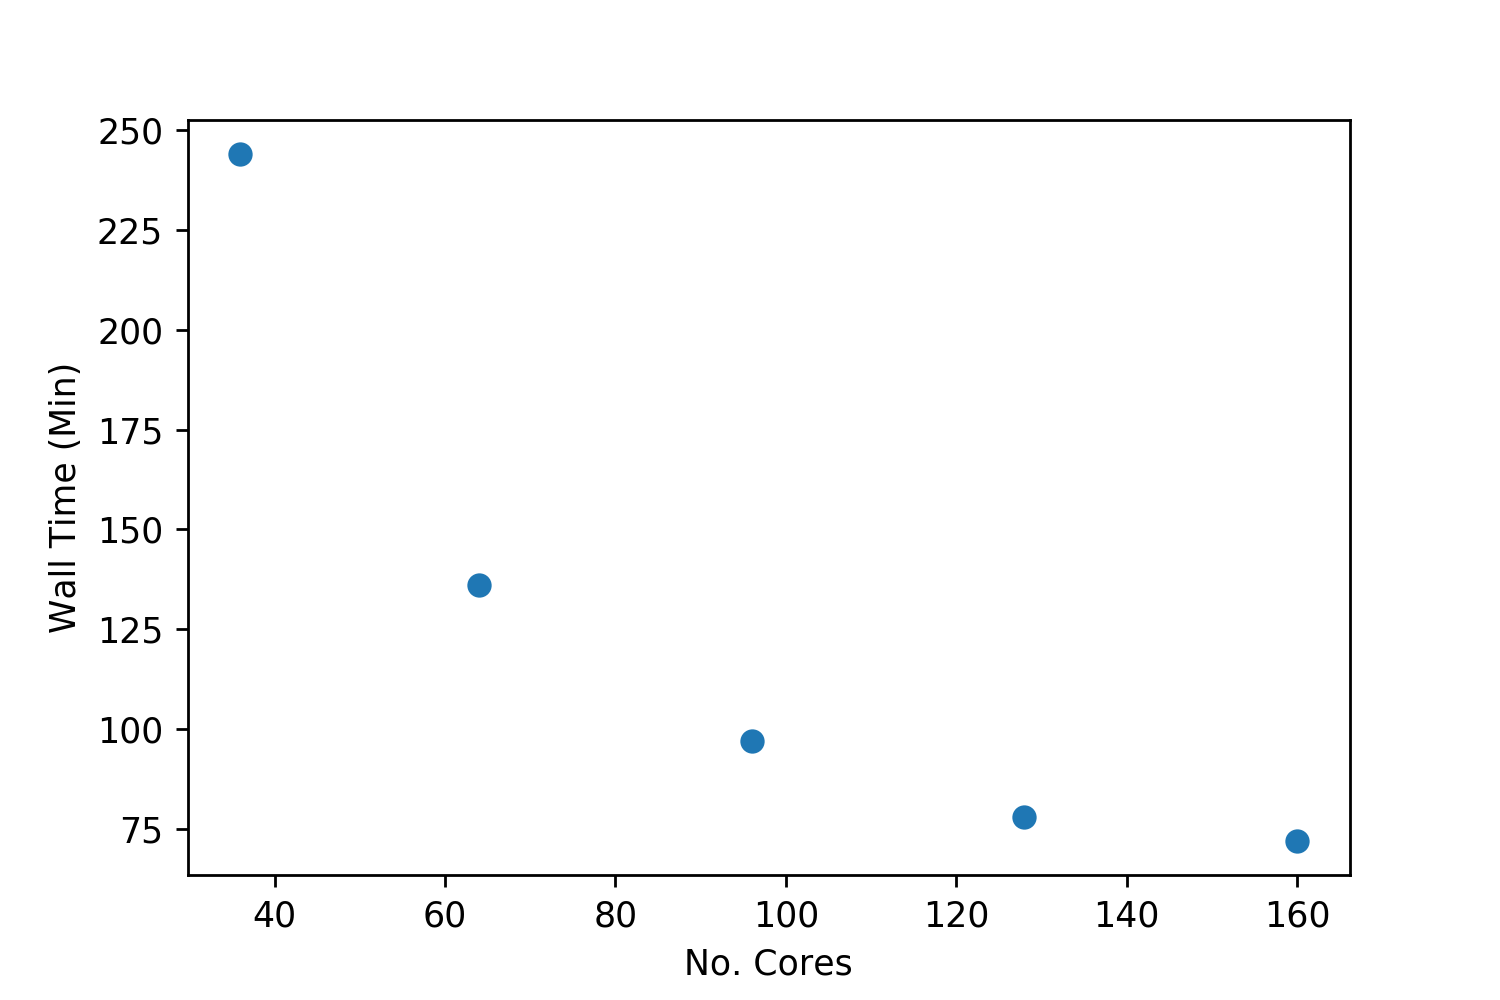
\includegraphics[height=8cm]{timepercores}}%
\caption{Scaling of the time necessary to complete the MCMC chain versus the number of cores used in the run.}
\label{fig1}
\end{figure}

The standard setup to run DES chains is 128 cores (4 nodes). We can see from both Table\ref{post} and Figure\ref{fig1} that this configuration is optimal to our problem, which seeks to balance speeding up the runs keeping a reasonable walltime. We observe that while going above 4 nodes does decrease the time necessary for the chain to complete, it starts to saturate at 5 nodes and there is no advantage in keep increasing the number of nodes. We conclude that the best scaling to reduce the walltime is to use 128 cores per run. 


\end{small}

\end{document}
